\begin{frame}{Rückblick~\textendash~Problemstellung}
    \begin{itemize}
        \item Einführung in Quanten-Computing
        \item Problem von Deutsch \& Deutsch-Jozsa-Algorithmus
        \item Starke indizien für Quantenüberlegenheit (Quantum Supremacy)
        \item Shor's-Algorithmus
        \item \textbf{Was nun?}
    \end{itemize}

    \note{
        Quantenüberlegenheit: Quantencomputer schlägt klassische Rechner in spezifischen Aufgaben - jedoch noch nicht eindeutig bewiesen.\newline
        \newline
        Wenn ein Quantencomputer gebaut werden kann um Shor's-Algorithmus effektiv laufen zu lassen, können klassische Verschlüsselungssysteme welche auf der Primfaktorzerlegung basieren einfach geknackt werden (e.g., RSA, ECC).
    }
\end{frame}

\begin{frame}{Entwicklung quanten-resistenter Einwegfunktionen}
    \begin{itemize}
        \item {
            \textbf{Learning with Errors (LWE)~\&~Gitterprobleme}\newline
            \(\rightarrow\) mutmasslich NP-Schwer~\&~quanten-resistent
        }
        \item \textbf{Verfahren von Regev} (Odded Regev)
        \item Cryptographic Suite for Algebraic Lattices (CRYSTALS) Projekt
        \item CRYSTALS entwickelt \textbf{Kyber} (Verschlüsselung)~\&~Dilithium (Signaturen)
        \item Module-Lattice-Based Key-Encapsulation Mechanism (ML-KEM)
    \end{itemize}

    \note{
        Es stellt sich heraus, dass sich dazu Learning with Errors (LWE) in kombination mit Gitterprblemen eignet.\newline
        \newline
        Diese Methode wurde 2005 erstmals von Odded Regev verwendet, um ein Quanten-Resistentes Verschlüsselungsverfahren zu entwerfen. 2018 erhielt Regev für diese Arbeit den Gödel-Preis.\newline
        \newline
        Das Verfahren wurde im Projekt CRYSTALS von einem Kryptografen-Team unter dem Namen "Kyber" weiterentwickelt und erstmals 2017 veröffentlicht.\newline
        \newline
        Kyber wurde von der NIST standartisiert und 2024 unter dem Namen Module-Lattice-Based Key-Encapsulation Mechanism (kruz: ML-KEM) veröffentlicht.\newline
    }
\end{frame}


\begin{frame}{Übersicht}
    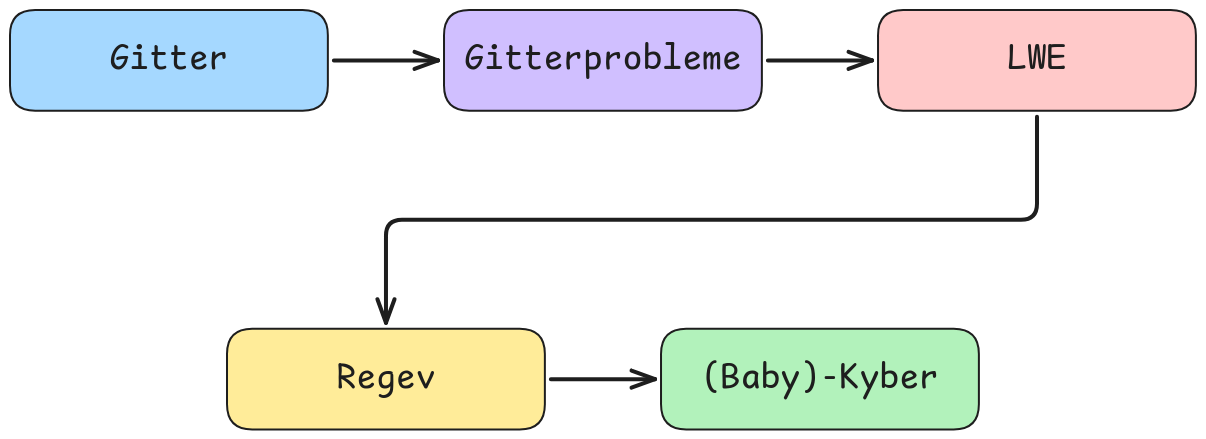
\includegraphics[width=\textwidth]{../assets/postquantum_lectures_overview.excalidraw.png}
    \note{
        In diesem Vortrag erarbeiten wir die mathematischen Grundlagen zum Verstehen von Gitterproblemen, Learning with Errors und wie man aus ihnen ein Verschlüsselungssystem entwerfen kann.\newline
        \newline
        Im nächsten Vortag schauen wir uns das Verfahren von Regev und Baby-Kyber an, eine vereinfachte Version von Kyber.
    }
\end{frame}